%%%%%%%%%%%%%%%%%%%%%%%%%%%%%%%%%%%%%%%%%%%%%%%%%%%
%
%  New template code for TAMU Theses and Dissertations starting Fall 2016.
%
%
%  Original Author: Sean Zachary Roberson
%  This version adapted for URS by Parasol lab.
%  Adapted from version 3.16.10, which was last updated on 9/29/2016.
%  URS adaptation last updated 1/9/2017.
%\part{title}
%%%%%%%%%%%%%%%%%%%%%%%%%%%%%%%%%%%%%%%%%%%%%%%%%%%

\documentclass[12pt]{report}

%These next lines change the font. Fixes for certain
%fonts will be implemented in a future release.

%Comment this line if you do not wish to use Times
%New Roman. The font used will then be the LaTeX
%default of Computer Modern.
\usepackage{times}
%\usepackage{cmbright}
\usepackage[T1]{fontenc}

%Do not change these settings. The geometry package
%Adjusts the margins to those specified by the Thesis
%Manual.
\usepackage[letterpaper]{geometry}
\geometry{verbose,tmargin=1.25in,bmargin=1.25in,lmargin=1.4in,rmargin=1.15in}
\usepackage[doublespacing]{setspace}
\usepackage{packages/tocloft}
\usepackage[rm, tiny, center, compact]{packages/titlesec}
\usepackage{indentfirst}
\usepackage{etoolbox}

\usepackage{packages/tocvsec2}
\usepackage[titletoc]{packages/appendix}
\usepackage{packages/appendix}
\usepackage{tamuconfig}

\usepackage{rotating}

%These are common AMS packages. Many LaTeX documents
%have these packages declared in their preambles.
\usepackage{amsmath, amsthm}

%This package allows for the use of graphics in the
%document.
\usepackage{graphicx}

%It is best practice to keep all your pictures in
%one folder inside the main directory in which your
%TeX file is kept. Here the folder is named "graphic."
%Replace the name here with your folder's name, if needed.
%The period is needed due to relative referencing.
\graphicspath{ {./graphic/} }

%If needed, this will allow you to add the word "Page"
%to extra pages on your front matter lists.
\usepackage{afterpage}

%This is from the mdwtools package; it fixes some
%footnote commands and allows you to have footnotes in
%tables via the savenotes environment.
\usepackage{footnote}
\usepackage{chngcntr}
\counterwithout{footnote}{chapter}


% Added to fix issues with pdf searching in some versions of LaTeX
%\usepackage[T1]{fontenc}\usepackage{lmodern}
%%%%%%%%%%%%%%%%%%%%%%%%%%%%%

% Hyperref setup below.  You should be able to get away with using uncommenting just the first line.
%\usepackage[hidelinks]{hyperref}

% if \usepackage[hidelinks]{hyperref} doesn't work try this.
%\usepackage{hyperref}  % Hidelinks is an option that removes link visiability.  TAMU Thesis Offices prefers to not see the links. But often doesn't work.
%
%\hypersetup{
%    colorlinks=true,
%    linkcolor=black,
%    citecolor=black,
%    filecolor=black,
%    urlcolor=black,
%}
%%%%%%%  End of hyperref setup.  One of these two options should work, but my motto with hyperref is when in doubt, comment it out!
%%%%%%%%%  This hopefully fixes the problem with vertical spacing of section headings at the top of the page..  Commented out in 1.0.7
% \preto\section{%
% \ifnum\value{section}>0\addtocontents{toc}{\vskip-6pt}\fi
% }
% \preto\subsection{%
% \ifnum\value{subsection}=0\addtocontents{toc}{\vskip-6pt}\fi
% \ifnum\value{subsection}>0\addtocontents{toc}{\vskip-6pt}\fi
% }
%%%%%%%%%%%%%%%%%%%%%%%%%%%%%%%%%%%%%%%%%%%%%%%%%%%%%%

\begin{document}

%The title of your document goes here.
%Spacing may need to be adjusted if your title is long
%and pushes the copyright off the page.
\renewcommand{\title}{[The Title of Your Thesis Goes In This Space To Let Us Know What Your Document is About]}

\newcommand{\abstracttitle}{[The Title of Your Thesis Goes Here Using Title Case Formatting]}

\renewcommand{\author}{[Insert Name]}

%Your department name goes here.
\newcommand{\department}{[Insert Primary Major]}

\newcommand{\program}{Undergraduate Research Scholar}

\newcommand{\ursadvisor}{[Advisor Name]}
\newcommand{\advisordepartment}{[Advisor Department]}

% Doesn't change until next year.
\newcommand{\ursmonth}{May}
\newcommand{\ursyear}{2018}

%\titleformat{\chapter}[display]
%{\normalfont\bfseries\filcenter}{\chaptertitlename\
%\thechapter}{14pt}{\fontsize{14pt}{12pt}}

%%%%%%%%%%%%%%%%%%%%%%%%%%%%%%%%%%%%%%%%%%%%%%%%%%%
%
%  New template code for TAMU Theses and Dissertations starting Fall 2016.
%
%
%  Original Author: Sean Zachary Roberson
%  This version adapted for URS by Parasol lab.
%  Adapted from version 3.16.10, which was last updated on 9/29/2016.
%  URS adaptation last updated 1/9/2017.
%
%%%%%%%%%%%%%%%%%%%%%%%%%%%%%%%%%%%%%%%%%%%%%%%%%%%

%%%%%%%%%%%%%%%%%%%%%%%%%%%%%%
%% TITLE PAGE
%% The values get updated automatically.  Please do not make changes to this file other than adding/deleting committee members where necessary.
%%%%%%%%%%%%%%%%%%%%%%%%%%%%%%

\providecommand{\tabularnewline}{\\}



\begin{titlepage}

\begin{center}
\MakeUppercase{\textbf{\large{\title}}}
\vspace{4em}

An Undergraduate Research Scholars Thesis

by

\MakeUppercase{\author}

\vspace{4em}

\begin{singlespace}

Submitted to the Undergraduate Research Scholars program at\\
Texas A\&M University \\

in partial fulfillment of the requirements for the designation as an\\

\end{singlespace}

\vspace{2em}
\MakeUppercase{\program}
\par\end{center}

\begin{singlespace}
  \begin{tabular}{ll}
    & \tabularnewline & \cr
  \end{tabular}
\end{singlespace}

\begin{center}
  \vspace{\baselineskip}
  \begin{singlespace}
    Approved by Research Advisor:\hfill~Dr.~\ursadvisor
  \end{singlespace}
  \vspace{\baselineskip}
\end{center}


\begin{center}
\ursmonth \hspace{2pt} \ursyear

\vspace{3em}

Major: \department \par

\vspace{3em}

\par\end{center}
\end{titlepage}
\pagebreak{}




 % This is simply a file that formats and adds your titlepage, please do not edit this unless you have a specific need. .

%%%%%%%%%%%%%%%%%%%%%%%%%%%%%%%%%%%%%%%%%%%%%%%%%%%
%
%  New template code for TAMU Theses and Dissertations starting Fall 2016.
%
%
%  Original Author: Sean Zachary Roberson
%  This version adapted for URS by Parasol lab.
%  Adapted from version 3.16.10, which was last updated on 9/29/2016.
%  URS adaptation last updated 1/9/2017.
%
%%%%%%%%%%%%%%%%%%%%%%%%%%%%%%%%%%%%%%%%%%%%%%%%%%%
%%%%%%%%%%%%%%%%%%%%%%%%%%%%%%%%%%%%%%%%%%%%%%%%%%%%%%%%%%%%%%%%%%%%%%
%%       TABLE OF CONTENTS
%%%%%%%%%%%%%%%%%%%%%%%%%%%%%%%%%%%%%%%%%%%%%%%%%%%%%%%%%%%%%%%%%%%%%
% single-space sections in Table of Contents  - commented in version 1.7
%\renewcommand{\cftsecafterpnum}{\vskip0.5\baselineskip}
%\renewcommand{\cftsubsecafterpnum}{\vskip0.5\baselineskip}
%\renewcommand{\cftsubsubsecafterpnum}{\vskip0.5\baselineskip}
%%%%%%%%%%%%%%%%%%%%%%%%%%%%%%%%%%%%%%%%%%%%%%%%%%%

\phantomsection
\pagenumbering{gobble}
%\addcontentsline{toc}{chapter}{TABLE OF CONTENTS}

\begin{singlespace}
  \renewcommand\contentsname{\normalfont}
  {\centerline{{\textbf{\large{TABLE OF CONTENTS}}}}}

%\setcounter{tocdepth}{4} % This puts \subsubsection[]{×} in your List of Tables.  The default is 3.

\setcounter{tocdepth}{1}

%%%%%%%%%%%%%  Adds Page above the page number in TOC
\setlength{\cftaftertoctitleskip}{1em}
\renewcommand{\cftaftertoctitle}{%
\hfill{\normalfont {Page}\par}}


\tableofcontents

%\addtocontents{toc}{\protect\afterpage{~\hfill\normalfont{Page}\par\medskip}}
\end{singlespace}

\pagebreak{}
  % This adds the table of contents, please do not edit this unless you have a specific need.
%%%%%%%%%%%%%%%%%%%%%%%%%%%%%%%%%%%%%%%%%%%%%%%%%%%
%
%  New template code for TAMU Theses and Dissertations starting Fall 2016.
%
%
%  Original Author: Sean Zachary Roberson
%  This version adapted for URS by Parasol lab.
%  Adapted from version 3.16.10, which was last updated on 9/29/2016.
%  URS adaptation last updated 1/9/2017.
%
%%%%%%%%%%%%%%%%%%%%%%%%%%%%%%%%%%%%%%%%%%%%%%%%%%%
%%%%%%%%%%%%%%%%%%%%%%%%%%%%%%%%%%%%%%%%%%%%%%%%%%%%%%%%%%%%%%%%%%%%%
%%                           ABSTRACT
%%%%%%%%%%%%%%%%%%%%%%%%%%%%%%%%%%%%%%%%%%%%%%%%%%%%%%%%%%%%%%%%%%%%%

\chapter*{ABSTRACT}

\addcontentsline{toc}{chapter}{ABSTRACT} % Needs to be set to part, so the TOC doesnt add 'CHAPTER ' prefix in the TOC.

\pagestyle{plain} % No headers, just page numbers
\pagenumbering{arabic} % Arabic numerals
\setcounter{page}{1}
\begin{center}

\begin{singlespace}
\abstracttitle
\end{singlespace}
\vspace{2em}
\begin{singlespace}
\author \\
Department of \department \\
Texas A\&M University \\
\end{singlespace}
\vspace{2em}
\begin{singlespace}
Research Advisor: Dr. \ursadvisor \\
Department of \advisordepartment \\
Texas A\&M University \\
\end{singlespace}
\end{center}
\vspace{2em}

\indent This is the first numbered page Arabic numeral 1. Page
numbers are outside the 1 inch margins (on all sides), at the bottom of the page and centered; everything else is inside the margins. No bold on this page (Exception: heading ABSTRACT is bold if major headings are bold. Text begins two double spaces below the major heading. Recommended length of
text is no more than 350 words. Vertical spacing is double spaced or
space-and-a-half. (\emph{This \LaTeX ~ template applies double space for this
ABSTRACT.}) The same margin settings and text alignment are followed else where
in this thesis. There should be no numbered references or formal citations in
the ABSTRACT.

The content of this ABSTRACT provides a complete, succinct snapshot of the
research, addressing the purpose, methods, results, and conclusions of the
research. As a result, it should stand alone without any formal citations or
references to chapters/sections of the work. To accommodate with a variety of online database, images or complex equations should also be avoided.

The next pages are Dedication, Acknowledgments, and Nomenclature.


\pagebreak{}

%%%%%%%%%%%%%%%%%%%%%%%%%%%%%%%%%%%%%%%%%%%%%%%%%%%
%
%  New template code for TAMU Theses and Dissertations starting Fall 2016.
%
%
%  Original Author: Sean Zachary Roberson
%  This version adapted for URS by Parasol lab.
%  Adapted from version 3.16.10, which was last updated on 9/29/2016.
%  URS adaptation last updated 1/9/2017.
%
%%%%%%%%%%%%%%%%%%%%%%%%%%%%%%%%%%%%%%%%%%%%%%%%%%%
%%%%%%%%%%%%%%%%%%%%%%%%%%%%%%%%%%%%%%%%%%%%%%%%%%%%%%%%%%%%%%%%%%%%%%
%%                           DEDICATION
%%%%%%%%%%%%%%%%%%%%%%%%%%%%%%%%%%%%%%%%%%%%%%%%%%%%%%%%%%%%%%%%%%%%%
\chapter*{DEDICATION}
\addcontentsline{toc}{chapter}{DEDICATION}  % Needs to be set to part, so the TOC doesnt add 'CHAPTER ' prefix in the TOC.


\begin{center}
\vspace*{\fill}
To my mother, my father, my grandfather, and my grandmother. To see what happens with multiple lines, I extend this next part into a second line.
\vspace*{\fill}
\end{center}

\pagebreak{}

%%%%%%%%%%%%%%%%%%%%%%%%%%%%%%%%%%%%%%%%%%%%%%%%%%%
%
%  New template code for TAMU Theses and Dissertations starting Fall 2016.
%
%
%  Original Author: Sean Zachary Roberson
%  This version adapted for URS by Parasol lab.
%  Adapted from version 3.16.10, which was last updated on 9/29/2016.
%  URS adaptation last updated 1/9/2017.
%
%%%%%%%%%%%%%%%%%%%%%%%%%%%%%%%%%%%%%%%%%%%%%%%%%%%


%%%%%%%%%%%%%%%%%%%%%%%%%%%%%%%%%%%%%%%%%%%%%%%%%%%%%%%%%%%%%%%%%%%%%%
%%                           ACKNOWLEDGMENTS
%%%%%%%%%%%%%%%%%%%%%%%%%%%%%%%%%%%%%%%%%%%%%%%%%%%%%%%%%%%%%%%%%%%%%
\chapter*{ACKNOWLEDGMENTS}
\addcontentsline{toc}{chapter}{ACKNOWLEDGMENTS}  % Needs to be set to part, so the TOC doesnt add 'CHAPTER ' prefix in the TOC.


\indent This section is also optional, limited to four pages. It must follow the Dedication Page (or Abstract, if no Dedication). If listing preliminary pages in Table of Contents, include Acknowledgments. Heading (\MakeUppercase{Acknowledgments}) is bold if major headings are bold. It should be in same type size and style as text. So does vertical spacing, paragraph style, and margins. Also, ensure that the spelling of ``acknowledgments'' matches throughout the text and the table of contents.

\pagebreak{}

%%%%%%%%%%%%%%%%%%%%%%%%%%%%%%%%%%%%%%%%%%%%%%%%%%%
%
%  New template code for TAMU Theses and Dissertations starting Fall 2016.
%
%
%  Original Author: Sean Zachary Roberson
%  This version adapted for URS by Parasol lab.
%  Adapted from version 3.16.10, which was last updated on 9/29/2016.
%  URS adaptation last updated 1/9/2017.
%
%%%%%%%%%%%%%%%%%%%%%%%%%%%%%%%%%%%%%%%%%%%%%%%%%%%

%%%%%%%%%%%%%%%%%%%%%%%%%%%%%%%%%%%%%%%%%%%%%%%%%%%%%%%%%%%%%%%%%%%%%%
%%                           NOMENCLATURE
%%%%%%%%%%%%%%%%%%%%%%%%%%%%%%%%%%%%%%%%%%%%%%%%%%%%%%%%%%%%%%%%%%%%%

\chapter*{NOMENCLATURE}
\addcontentsline{toc}{chapter}{NOMENCLATURE}  % Needs to be set to part, so the TOC doesnt add 'CHAPTER ' prefix in the TOC.

%A note about aligning: These entries will align
%themselves according to the ampersand (&).
%No extra spaces are needed, as seen in some of
%the entries below.
\vspace{-0.5in}
	\begin{table}[htbp]
	    \begin{tabular}{@{}p{0.33\textwidth} p{0.62\textwidth}@{}}
		B/CS		&	Bryan and College Station\\	[2ex] %[2ex] provides double space between each row
		TAMU			&	Texas A\&M University\\	[2ex]
		SDCC & San Diego Comic-Con\\ [2ex]
		EVIL & Every Villain is Lemons\\ [2ex]
		EPCC & Educator Preparation and Certification Center at Texas A\&M University - San Antonio\\ [2ex]
		FFT & Fast Fourier Transform\\ [2ex]
		ARIMA & Autoregressive Integrated Moving Average\\ [2ex]
		%XXXXXXXX		&	This is an optional page. Random word to test how long the sentence can be? This is just for test purpose. The current setting aims to align left/right margin same as all other pages.\\	[2ex]
	    \end{tabular}%
	\end{table}

\pagebreak{}


%%%%%%%%%%%%%%%%%%%%%%%%%%%%%%%%%%%%%%%%%%%%%%%%%%%
%
%  New template code for TAMU Theses and Dissertations starting Fall 2016.
%
%
%  Original Author: Sean Zachary Roberson
%  This version adapted for URS by Parasol lab.
%  Adapted from version 3.16.10, which was last updated on 9/29/2016.
%  URS adaptation last updated 1/9/2017.
%
%%%%%%%%%%%%%%%%%%%%%%%%%%%%%%%%%%%%%%%%%%%%%%%%%%%
%%%%%%%%%%%%%%%%%%%%%%%%%%%%%%%%%%%%%%%%%%%%%%%%%%%%%%%%%%%%%%%%%%%%%%
%%                           LIST OF FIGURES
%%%%%%%%%%%%%%%%%%%%%%%%%%%%%%%%%%%%%%%%%%%%%%%%%%%%%%%%%%%%%%%%%%%%%

\phantomsection
\addcontentsline{toc}{chapter}{LIST OF FIGURES}

\renewcommand{\cftloftitlefont}{\center\bf\large\MakeUppercase}

\setlength{\cftbeforeloftitleskip}{-12pt} %% Positions the LOF title vertically to match the chapter titles
\renewcommand{\cftafterloftitleskip}{12pt}


\renewcommand{\cftafterloftitle}{%
\\[4em]\mbox{}\hspace{2pt}FIGURE\hfill{\normalfont Page}\vskip\baselineskip}

\begingroup


\begin{center}
\begin{singlespace}
%% These values make the lof table entries appear double spaced between.
\setlength{\cftbeforechapskip}{0.4cm}
\setlength{\cftbeforesecskip}{0.30cm}
\setlength{\cftbeforesubsecskip}{0.30cm}
\setlength{\cftbeforefigskip}{0.4cm}
\setlength{\cftbeforetabskip}{0.4cm}

\listoffigures

\end{singlespace}
\end{center}

\pagebreak{}
  % This adds the list of figures, this is optional. To remove, add a comment '%' at the beggining of the line.
%%%%%%%%%%%%%%%%%%%%%%%%%%%%%%%%%%%%%%%%%%%%%%%%%%%
%
%  New template code for TAMU Theses and Dissertations starting Fall 2016.
%
%
%  Original Author: Sean Zachary Roberson
%  This version adapted for URS by Parasol lab.
%  Adapted from version 3.16.10, which was last updated on 9/29/2016.
%  URS adaptation last updated 1/9/2017.
%
%%%%%%%%%%%%%%%%%%%%%%%%%%%%%%%%%%%%%%%%%%%%%%%%%%%
%%%%%%%%%%%%%%%%%%%%%%%%%%%%%%%%%%%%%%%%%%%%%%%%%%%%%%%%%%%%%%%%%%%%%%
%%                           lIST OF TABLES
%%%%%%%%%%%%%%%%%%%%%%%%%%%%%%%%%%%%%%%%%%%%%%%%%%%%%%%%%%%%%%%%%%%%%%
%
\phantomsection
\addcontentsline{toc}{chapter}{LIST OF TABLES}

\renewcommand{\cftlottitlefont}{\center\bf\large\MakeUppercase}

\setlength{\cftbeforelottitleskip}{-12pt} %% Positions the LOT title vertically to match the chapter titles

%Note that the similar parameter in the LOF is 12pt; this
%is intentional to make the spacing between the headers
%and the first entry look consistent.
\renewcommand{\cftafterlottitleskip}{1pt}


\renewcommand{\cftafterlottitle}{%
\\[4em]\mbox{}\hspace{2pt}TABLE\hfill{\normalfont Page}\vskip\baselineskip}

\begin{center}
\begin{singlespace}

%% These values make the lot table entries appear double spaced between.
\setlength{\cftbeforechapskip}{0.4cm}
\setlength{\cftbeforesecskip}{0.30cm}
\setlength{\cftbeforesubsecskip}{0.30cm}
\setlength{\cftbeforefigskip}{0.4cm}
\setlength{\cftbeforetabskip}{0.4cm}

\listoftables

\end{singlespace}
\end{center}
\endgroup
\pagebreak{}  % Need this for the pagenumbering to be correct.
  % This adds the list of tables, this is optional. To remove, add a comment '%' at the beginning of the line.

%%%%%%%%%%%%%%%%%%%%%%%%%%%%%%%%%%%%%%%%%%%%%%%%%%%
%
%  New template code for TAMU Theses and Dissertations starting Fall 2016.
%
%
%  Original Author: Sean Zachary Roberson
%  This version adapted for URS by Parasol lab.
%  Adapted from version 3.16.10, which was last updated on 9/29/2016.
%  URS adaptation last updated 1/9/2017.
%
%%%%%%%%%%%%%%%%%%%%%%%%%%%%%%%%%%%%%%%%%%%%%%%%%%%
%%%%%%%%%%%%%%%%%%%%%%%%%%%%%%%%%%%%%%%%%%%%%%%%%%%%%%%%%%%%%%%%%%%%%%
%%                           SECTION I
%%%%%%%%%%%%%%%%%%%%%%%%%%%%%%%%%%%%%%%%%%%%%%%%%%%%%%%%%%%%%%%%%%%%%


\pagestyle{plain} % No headers, just page numbers
%\pagenumbering{arabic} % Arabic numerals
%\setcounter{page}{1}

\chapter{INTRODUCTION AND LITERATURE REVIEW}

\section{Read Me}

This template is derived from Texas A\&M University's Graduate \LaTeX thesis template found on their website on December 7th 2016. This template is to be used for Undergraduate
Research Scholars program at Texas A\&M. This template shows the many features of \LaTeX, with many more available to the user.

There are numerous guides, references, and tutorials available on the Internet to help you. If you are stuck, don't be afraid to conduct a Google search for your issue.

\subsection{Changes}

The changes made to the thesis template:
\begin{itemize}
  \item Added appropriate commands for the title, program, advisor, and department. Commands needed for the graduate thesis were removed.
  \item Modified the introduction of the template to be more accurate.
  \item Reformatted the title page to follow URS formatting rules.
  \item Reformatted the abstract page to follow URS formatting rules.
  \item Condensed the appendices to one page.
  \item Changed the section file names to chapter to be more concise naming convention.
  \item Added a makefile to compile the document.
  \item Various updates made for URS 2018. These include title formatting, TOC
    location, spelling/grammar errors, and more.
\end{itemize}

\subsection{Useful Resources and Websites}

Here are some useful tutorials and references on \LaTeX:
\begin{itemize}
  \item http://www.latex-tutorial.com/tutorials/
  \item http://www.cs.princeton.edu/courses/archive/spr10/cos433/Latex/latex-guide.pdf
  \item https://www.sharelatex.com/learn/Main\_Page
  \item https://tobi.oetiker.ch/lshort/lshort.pdf
  \item ftp://ftp.ams.org/pub/tex/doc/amsmath/short-math-guide.pdf
\end{itemize}

\subsection{Brief Usage of the Template}

This template is intended for use by STEM\footnote{Science, Technology, Engineering, and Mathematics. This is an example of a footnote. You can see that it is numbered and appended at the end of the page. Also, you can see the effect of having a multiline footnote.} students. If you are not a STEM student, this template is likely not for you.

The advantage of using this template over the Microsoft Word templates are
numerous. First, there is a lot of control granted to the user in how the
document looks. Of course, you are expected to still follow the guidelines set
forth in the URS Thesis Manual. This template takes care of the margins, heading requirements, and front matter ordering for you.


\subsection{Software to Install}

\textbf{TeXworks} and \textbf{TeXstudio} for Windows, MaxOS, and Linux are free software for compiling
your \LaTeX ~ document. To compile for this document, \textit{pdflatex} or \textit{xelatex} compiling engine
should be used. Make sure you are using bibtex for generating references. Do not use \textit{latex} compiling
engine if you are using png images because it will not know the size of the image.

\subsection{Procedure to Compile \LaTeX ~ Document}

This template (and consequently, your document) will be compiled using latex. To compile your document, do the following\footnote{Notice here that I also show off the itemize environment for unordered lists. Ordered lists use the enumerate environment.}:

\begin{itemize}
	\item In TeXstudio, go to the Tools menu, then select Commands, and click pdfLaTeX or XeLatex.
	\item In TeXworks, go to the Typeset menu and select pdfLaTeX or XeLatex.
	\item For other editors, consult the help files included with the editor.
\end{itemize}

If you are working in linux and want to use gnumake, make sure you have pdfLaTeX or XeLaTeX installed. To build on Linux, open a terminal, go to the
thesis directory and type \texttt{make} and hit enter. The document will build and create a file called \texttt{thesis.pdf} that will be your thesis.

To use make on MaxOS, commandline tools must be installed from Xcode. If it is not already install I do not recommend using this because
the Xcode is a large install and it might be advantageous to use one of the other mentioned methods.

\subsection{How to Fill This Document}
The document structure is organized in the main .tex file, thesis.tex,
which has the same name as the output PDF file. Content in each section is in the data folder. You can open the .tex files under the data folder to modify. Four sections
are added initially. To add in more sections into the \LaTeX document, open the
thesis.tex file and go to \textbf{line 137} you can just delete the content in the data folder and fill your documents and then compile under thesis.tex.)

\subsection{Reference Usage and Example}

This subsection tests the usage of references. The book\cite{REALCAR} is
referred in this way. Actually, the option is available for you to change the
default way how reference appears. The default and most commonly used option
\cite{einstein} is displayed here \cite{Barn-JORVQ}.

Unrelated citations are referred here for the test of reference section only. If
you find that the reference has more items than you need \cite{WAGFJ}, question
marks will show up in place of a reference handle, like these
\cite{a-reference-thats-not-in-your-bib-file}.

\subsection{Where to Start}

Getting started in \LaTeX can be a daunting task. To get started I recommend getting your the information into the
preliminary pages (abstract, acknowledgements, dedication, and nomenclature) as a way to learning how to move around
the different files. The information in the preliminary pages is controlled by fields located in
the files thesis.tex, and it allows you to enter the information into the template a single time. To modify
the preliminary pages in this template, follow these steps:

\begin{enumerate}

  \item Open the file thesis.tex in your \LaTeX\ editor.
    \begin{enumerate}
      \item Locate the command \texttt{{\textbackslash}title} and type your thesis title there.
      \item Locate the command \texttt{{\textbackslash}author} and type your name there.
      \item Locate the command \texttt{{\textbackslash}program}. Do not change this, it is already correct.
      \item Locate the command \texttt{{\textbackslash}ursadvisor} and type your research advisor's name there. Do not put
            "Dr." before their name; the template will do this for you.
      \item Locate the command \texttt{{\textbackslash}department} and type your primary department. If you have a secondary
            department, it isn't necessary for you to include it. You do not need to include the text "Department of" before
            the department names; the template will do this for you.
      \item Locate the command \texttt{{\textbackslash}advisordepartment} and type your advisor's department there. Again,
            you do not need to add "Department of".
    \end{enumerate}
  \item Save the file thesis.tex and open abstract.tex in the data directory
  \item Type your abstract after the \texttt{{\textbackslash}indent}.  Remember that your abstract should be no longer than 350 words.
        Do not change anything else in the file. The rest of the file is formatting the abstract's header.

  \item Save the file abstract.tex and open dedication.tex in the data directory
  \item Type your dedication between the \texttt{{\textbackslash}begin\{center\}} and \texttt{{\textbackslash}end\{center\}}
        commands and between the \texttt{{\textbackslash}vspace*} commands. This section is optional, and if you do not wish
        to include it, comment out the line \texttt{{\textbackslash}\{data/dedication\}} on \textbf{line 124} of thesis.tex
        by placing a \texttt{\%\texttt} character before the line. This will completely remove the dedication page.

  \item Save the file dedication.tex and open acknowledgements.tex in the data directory
  \item Type your acknowledgments after the \texttt{{\textbackslash}indent} command. This section is optional, and if you do not wish
        to include it, comment out the line \texttt{{\textbackslash}\{data/acknowledgments\}} on \textbf{line 125} of thesis.tex
        by placing a \texttt{\%\texttt} character before the line. This will completely remove the acknowledgments page.

  \item Save the file acknowledgments.tex and open nomenclature.tex in the data directory
  \item Type your nomenclature between \texttt{{\textbackslash}begin\{tabular\}} and \texttt{{\textbackslash}end\{tabular\}}.
        Within the table the abbreviation will be to the left of the \& and what it means will be the right. Use the examples
        already provided if you need more clarification. This section is optional, and if you do not wish to include it,
        comment out the line \texttt{{\textbackslash}\{data/acknowledgments\}} on \textbf{line 126} of thesis.tex
        by placing a \texttt{\%\texttt} character before the line. This will completely remove the nomenclature page.
  \item Save the file nomenclature.tex.
  \item Compile the document from thesis.tex. This is considered the \texttt{main} file for your thesis document.
  \item thesis.pdf should now contain the changes you made to the template. If you received any error messages
        use google or other resources provided to figure out what they mean and how to correct them.
\end{enumerate}

\subsection{Equations, Formulas, and Other Really Cool Math Things That \LaTeX ~ Can Do}

Equations can be written in \LaTeX ~ in one of two ways. First, you can have material displayed inline by enclosing the desired statement in dollar signs. For example, $e^{i\pi}+1=0$ is an inline math expression. Some longer expressions, especially those including sums, integrals, or large operators and objects can be displayed centered on their own line. In this \textbf{math mode}, you enclose the desired material in square brackets. For example,

\[ \sum_{j = 1} ^n \int f_j \ dx = \int \sum_{j = 1} ^n f_j \ dx \]
is a math mode expression. We can also have a series of expressions aligned at a symbol. This is particularly useful when you are showing details in solving an equation or evaluating an integral. The next block shows off the \textit{align*} environment. We use it here to show a distributive property of set intersections over unions. Observe how each line is aligned to the biconditional symbol. This makes reading steps easier, since a reader can go line by line and determine why each step is justified.

\begin{align*}
x \in A \cap \bigcup_{j} B_j &\iff x \in A \ \wedge \ x \in \bigcup_{j} B_j \\
&\iff x \in A \ \wedge \ x \in B_k \ \text{ for some k} \\
&\iff x \in \bigcup_{j} A \cap B_j
\end{align*}

There are many more commands and features available, but this document is too small to contain them.\footnote{Yes, I pulled a Fermat. But really, a Google search will likely help you find what you need to do.} Many guides are available on the Internet for your use.

%Have some material about the align environments. Include also the eqn environment.

\subsection{A Test Subheading}

This is just a test.

\subsection{Another Test Subheading}
Hello, is it me you're looking for?

\subsection{Yet Another One}
She called me late last night to say she loved me so.

\subsection{No Surprises Here}
Insert another song lyric here.


%%%%%%%%%%%%%%%%%%%%%%%%%%%%%%%%%%%%%%%%%%%%%%%%%%%
%
%  New template code for TAMU Theses and Dissertations starting Fall 2016.
%
%
%  Original Author: Sean Zachary Roberson
%  This version adapted for URS by Parasol lab.
%  Adapted from version 3.16.10, which was last updated on 9/29/2016.
%  URS adaptation last updated 1/9/2017.
%
%%%%%%%%%%%%%%%%%%%%%%%%%%%%%%%%%%%%%%%%%%%%%%%%%%%
%%%%%%%%%%%%%%%%%%%%%%%%%%%%%%%%%%%%%%%%%%%%%%%%%%%%%%%%%%%%%%%%%%%%%%%
%%%                           SECTION II
%%%%%%%%%%%%%%%%%%%%%%%%%%%%%%%%%%%%%%%%%%%%%%%%%%%%%%%%%%%%%%%%%%%%%%


\chapter{PAGES WITH A FIGURE, A TABLE AND AN EQUATION}
\section{Figures: Placement, Size, and Captions}
This is a figure template.
\begin{figure}[ht]
\centering
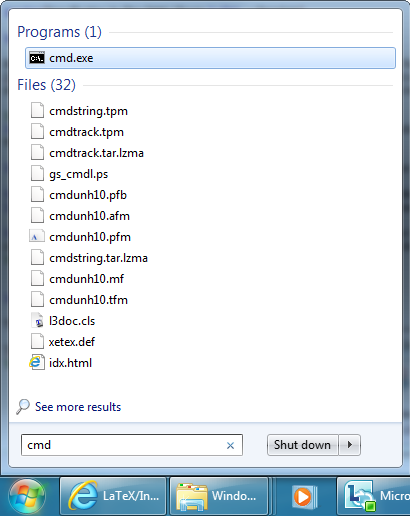
\includegraphics[scale=0.75]{TAMUthesis_CMD_windows.png}
\caption[The command line compiler in Windows.]{The command line compiler in Windows. It is not suggested that you compile using this method. See compilation instructions in the README.}

\label{fig:CMD_1}

\end{figure}

Figure (and table) titles should be consistent through the document. All
captions should be placed either above or below the object it describes. This is
done by placing the \textit{caption} in the correct place. While continued
figures are allowed by the URS Thesis Manual with proper continuation headings, it is not suggested that any continued figures be included in a \LaTeX\ document.

The figure below is taken from R. While there are packages available to import
graphics from R, MATLAB, and similar software, it is probably best to export
plots generated by these programs as a PNG file, and then import it via the
\textit{includegraphics} command. Figures must also be referenced in the body
text within 1 page of where the figure actually appears in the document.

\begin{figure}[ht]
	\centering
	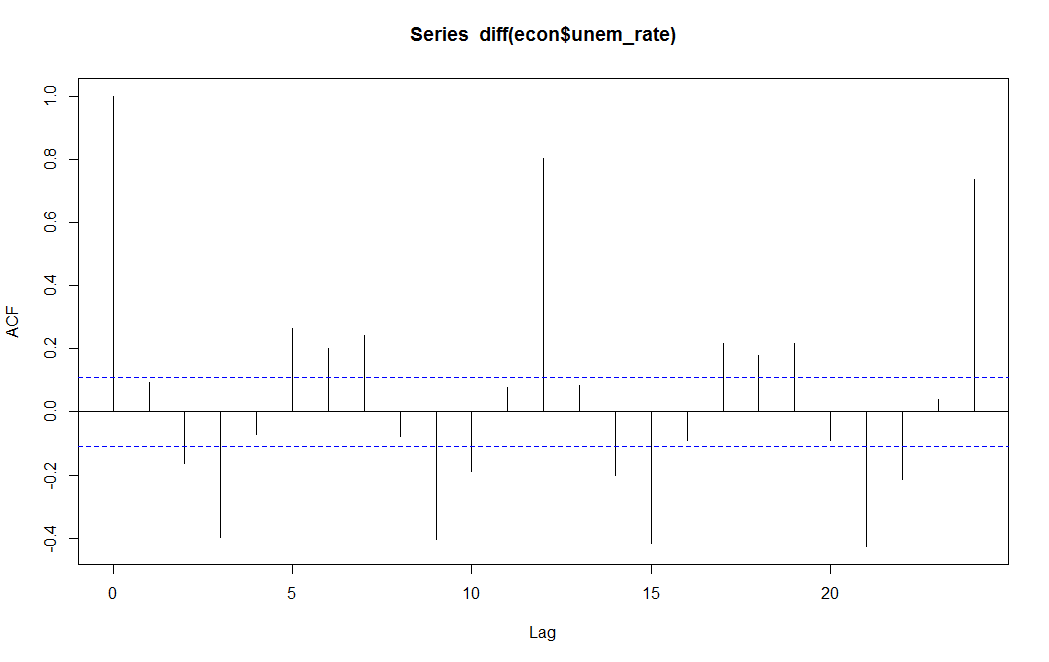
\includegraphics[scale=0.55]{UnemDiffACF.png}
	\caption{The autocorrelation function (ACF) of the differenced unemployment series. Seasonal adjustments may be needed.}
\end{figure}

\section{Table Placement, Size and Table Title}

Here is a table, displaying band and auxiliary scores from the 2011 Arcadia Festival of Bands held in Arcadia, CA \cite{ARCADIA}.

\begin{table}[h!]
	\centering

	\label{Band}
	\caption{Scores from the 2011 Arcadia Festival of Bands.}
        \vspace{1em}
	\begin{tabular}{|l|l|l|}
		\hline
		School Name & Band Score & Auxiliary Score \\ \hline
		Rancho Bernardo & 96.15 & 89.15 \\ \hline
		Mt. Carmel & 95.30 & 83.55 \\ \hline
		Riverside King & 93.85 & 91.75 \\ \hline
		Diamond Bar & 93.20 & 88.60 \\ \hline
		El Dorado & 92.80 & 95.45 \\ \hline
		Chino & 92.65 & 91.45 \\ \hline
		Henry J. Kaiser & 92.60 & 87.55 \\ \hline
		Glendora & 92.60 & 89.15 \\ \hline
		Montebello & 90.50 & 82.70 \\ \hline
		Mira Mesa & 89.65 & 91.50 \\ \hline
	\end{tabular}
\end{table}

The table is sorted by band score. There is more text here to demonstrate how
the template handles spacing between tables and body text. Also note how the
table caption is in a smaller font size than the body text.

\section{Equations}

The following format is recommended to be used to display equations.

%Make other examples.
\begin{equation} \label{Equ.2.1}
y=c_1\cos(t)+c_2\sin(t)
\end{equation}
\begin{equation} \label{Equ.2.2}
e^{it}=\cos(t)+i\sin(t)
\end{equation}

Equation \ref{Equ.2.1} is the general solution to the differential equation $y''+y=0$. In the source code, the \textit{ref} command allows you to refer to an equation by a label you created. References must be made after the equation has been created; attempting to refer to an equation before it is defined results in a question mark placeholder. Some more sample equations are below. Notice the first set below is not numbered.
%%
\begin{align*}
\log (x^n) &= \log (x \cdot x \cdot \ldots \cdot x) \\
&= \log x + \log x + \ldots + \log x \\
&= n \log x
\end{align*}
\begin{equation} \label{Equ.2.3}
X^T X \mathbf{u} = X^T \mathbf{y}
\end{equation}
\begin{equation}\label{Equ.2.4}
u(x, t) = \int_{-\infty}^{\infty} G(x, \tau) \exp\left(-\frac{(t-\tau)^2}{4kt}\right) \ d\tau
\end{equation}
\begin{gather}
\mathcal{L}(f) = \int_{0}^{\infty} e^{-st} f(t) \ dt \\
\begin{split} \label{Equ.2.5}
\mathcal{F}(f) = \frac{1}{2\pi}\int_{-\infty}^{\infty} e^{i \omega x} f(x) \ dx
\end{split}
\end{gather}

You can use labels to refer to equations you create. \ref{Equ.2.5} is the \textbf{Laplace transform} used extensively in differential equations. \ref{Equ.2.3} is the matrix representation of the \textbf{normal equations} used in least-squares regression.

To have equations without labels appearing the right margin, simply add an asterisk to the name of the environment (equation, align, etc.) when making the declaration.


\section{Theorems and Proofs: Examples}

This section will show an example usage of the theorem and proof environments, typically used for mathematics students. To use these environments, you must have the package \textbf{amsthm} declared in the preamble of your document. For this template, this is already declared in the main file. You may choose to remove this declaration if your document will not make use of theorems and proofs.

Theorems can be numbered, as the one below is, or you can force a different label to appear. For example, you can state the Bolzano-Weierstass theorem and have the names appear as the theorem label. See the examples below.

Sometimes you may have a theorem with multiple parts or multiple conditions. You can use other list environments, such as enumerate, inside the theorem environment declared to list these conditions. The final example at the end of this block shows this with the Invertible Matrix Theorem, which has several equivalent statements.

\renewcommand{\qedsymbol}{\rule{0.7em}{0.7em}}

\newtheorem{thm}{Theorem}
\begin{thm}
	Suppose $f$ is of class $\mathcal{C}^1$ and $g$ is of class $\mathcal{C}^2$, and that the compact set $D$ and its boundary satisfy the hypotheses of Green's Theorem.  Then
	\[ \iint \limits_D f\nabla^2 g \ dA = \oint_{\partial D} f(\nabla g) \cdot \mathbf{n} \ ds - \iint \limits_D \nabla f \cdot \nabla g \ dA . \]
\end{thm}

\begin{proof}
	Begin with the integral of $f\nabla g \cdot n$ taken over the boundary of D.  By the second vector form of Green's Theorem,
	\begin{align*}
	\oint_{\partial D} f\nabla g \cdot n \ ds &= \iint \limits_D \nabla \cdot (f\nabla g) \ dA \\
	&= \iint \limits_D f\nabla^2 g + \nabla f \cdot \nabla g \ dA.
	\end{align*}

	Rearranging yields the desired.
\end{proof}

\begin{thm}[Bolzano-Weierstrass]
	Every bounded real sequence has a convergent subsequence.
\end{thm}

\begin{thm}[Invertible Matrix Theorem\footnote{This is an incomplete list.}]
	For any square matrix $A$ with $n$ rows and columns, the following are equivalent.
	\begin{enumerate}
		\item $A$ is invertible.
		\item The equation $A\mathbf{x}=\mathbf{0}$ has only the trivial solution $\mathbf{x} = \mathbf{0}.$
		\item For any nonzero $\mathbf{b}, \ A\mathbf{x} = \mathbf{b}$ has exactly one solution.
		\item The columns of $A$ form a linearly independent set.
		\item Zero is not an eigenvalue of $A$.
		\item $A$ has full rank.
		\item The determinant of $A$ is not zero.
	\end{enumerate}
\end{thm}

There is currently no set format on how propositions and theorems should be laid out in the document. The idea is to remain consistent. It is best to not customize the appearance of theorems so that they can easily be distinguished from body text - just like figures, tables, and headings.

\section{Another Table Example}
For the sake of testing the appearance of the list of tables, a second table will be displayed here. This table displays a list of some major universities and their enrollments during fall 2015. This table is sorted in descending order of enrollment.
%The savenotes environment, loaded from the footnote package
%(which in turn is loaded from mdwtools)
%allows you to use footnotes in tables, if needed.
\begin{savenotes}
\begin{table}[h!]
	\centering
	\label{my-label}
	\caption{Some major universities and their fall 2015 enrollments.}
        \vspace{1em}
	\begin{tabular}{|l|l|l|}
		\hline
		School & City and State & Fall 2015 Enrollment  \\ \hline
		Texas A\&M University\footnote{Gig 'em!} & College Station, TX & 64,376  \\ \hline
		Ohio State University\footnote{This number describes enrollments at the Columbus campus; enrollments at regional campuses in Lima, Mansfield, Marion, Newark, and Wooster are not counted.} & Columbus, OH & 58,322 \\ \hline
		Iowa State University & Ames, IA & 36,001 \\ \hline
		University of California, San Diego & La Jolla, CA & 33,735   \\ \hline
		University of West Florida & Pensacola, FL & 12,798 \\ \hline
		Massachusetts Institute of Technology & Cambridge, MA & 11,319   \\ \hline
	\end{tabular}
\end{table}
\end{savenotes}

Naturally, tables and footnotes do not go together. If you attempted to write a footnote inside a table, there will be nothing at the bottom of the page, yet the footnote marker will still appear. To remedy this, the \textit{footnote} package has been loaded from the \textit{mdwtools} package. Check your TeX distribution to see if \textit{mdwtools} is installed. See the source code for how this is implemented.

%%%%%%%%%%%%%%%%%%%%%%%%%%%%%%%%%%%%%%%%%%%%%%%%%%%
%
%  New template code for TAMU Theses and Dissertations starting Fall 2016.
%
%
%  Original Author: Sean Zachary Roberson
%  This version adapted for URS by Parasol lab.
%  Adapted from version 3.16.10, which was last updated on 9/29/2016.
%  URS adaptation last updated 1/9/2017.
%
%%%%%%%%%%%%%%%%%%%%%%%%%%%%%%%%%%%%%%%%%%%%%%%%%%%
%%%%%%%%%%%%%%%%%%%%%%%%%%%%%%%%%%%%%%%%%%%%%%%%%%%%%%%%%%%%%%%%%%%%%%
%%                           SECTION III
%%%%%%%%%%%%%%%%%%%%%%%%%%%%%%%%%%%%%%%%%%%%%%%%%%%%%%%%%%%%%%%%%%%%%



\chapter{VERY, VERY, VERY LONG TITLE THAT FLOWS INTO A SECOND LINE FOR THE SAKE OF EXAMPLE}

Notice that the title of this section is long - much longer than the others. When you have long section titles, this template takes care of double spacing the lines in the title. If the title is long to fit in the table of contents, the template will single space the title.

\section{Yet Another Table}

Another table is placed here to show the effect of having tables in multiple sections. The list of tables should still double space between table titles, while single spacing long table titles.

%Fix table labeling.
\begin{table}[h!]
	\centering
	\caption{San Japan attendance. Data is taken from \cite{ANCONS}. I intentionally make the title of this table long so the single space effect is seen in the list of tables.}
        \vspace{1em}
	\begin{tabular}{|l|l|}
		\hline
		Dates & Attendance  \\ \hline
		August 8-10, 2008 & 3,523  \\ \hline
		August 14-16, 2009 & 4,003 \\ \hline
		July 9-11, 2010 & 5,049 \\ \hline
		August 5-7, 2011 & 6,891  \\ \hline
		August 10-12, 2012 & 9,464  \\ \hline
		August 16-18, 2013 & 11,077  \\ \hline
		July 18-20, 2014 & 14,686 \\ \hline
		July 31-August 2, 2015 & 18,411  \\ \hline
	\end{tabular}
\end{table}

You may be wondering why San Japan was chosen. There are a few reasons as to why I did this:

\begin{enumerate}
\item It is one of the fastest-growing anime conventions in Texas.
\item Filler.
\item I wanted a good variety of table examples.
\item Because conventions are cool.
\end{enumerate}

The \textit{enumerate} environment was used to generated an ordered list above.

\section{Section Test Example}
We insert another figure here, just for kicks.

\begin{figure}[h!]
	\centering
	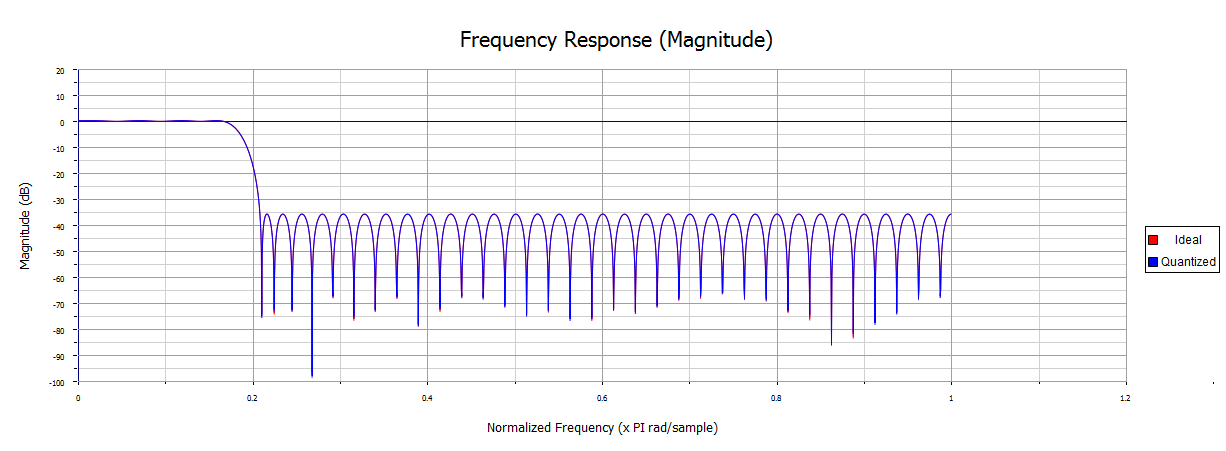
\includegraphics[scale=0.5]{LowPass_Filter_Design.png}
	\caption{A low pass filter design.}
\end{figure}

%%%%%%%%%%%%%%%%%%%%%%%%%%%%%%%%%%%%%%%%%%%%%%%%%%%
%
%  New template code for TAMU Theses and Dissertations starting Fall 2016.
%
%
%  Original Author: Sean Zachary Roberson
%  This version adapted for URS by Parasol lab.
%  Adapted from version 3.16.10, which was last updated on 9/29/2016.
%  URS adaptation last updated 1/9/2017.
%
%%%%%%%%%%%%%%%%%%%%%%%%%%%%%%%%%%%%%%%%%%%%%%%%%%%
%%%%%%%%%%%%%%%%%%%%%%%%%%%%%%%%%%%%%%%%%%%%%%%%%%%%%%%%%%%%%%%%%%%%%%
%%                           SECTION IV
%%%%%%%%%%%%%%%%%%%%%%%%%%%%%%%%%%%%%%%%%%%%%%%%%%%%%%%%%%%%%%%%%%%%%



\chapter{SUMMARY AND CONCLUSIONS \label{cha:Summary}}

**Some text/figure here**

\section{Challenges}
Section here is to test toc display only.

\section{Further Study}
Section here is to test toc display only.



%The next line is the format for inserting new sections.
%Replace the name "newsection"  with the name of your
%new section file.
%\include{data/newsection}


%fix spacing in bibliography, if any...
%%%%%%%%%%%%%%%%%%%%%%%%%%%%%%%%%%%%%%%%%%%%%%%%%%%%%%%%%%%%%
%\let\oldbibitem\bibitem
%\renewcommand{\bibitem}{\setlength{\itemsep}{0pt}\oldbibitem}
%%%%%%%%%%%%%%%%%%%%%%%%%%%%%%%%%%%%%%%%%%%%%%%%%%%%%%%%%%%%%%%
%The bibliography style declared is the IEEE format. If
%you require a different style, see the document
%bibstyles.pdf included in this package. This file,
%hosted by the University of Vienna, shows several
%bibliography styles and examples of in-text citation
%and a references page.

\phantomsection
\addcontentsline{toc}{chapter}{REFERENCES}

\renewcommand{\bibname}{{\large\rm\bf REFERENCES}}
%This file is a .bib database that contains the sources.
\bibliography{data/myReference}
\bibliographystyle{ieeetr}

%This next line includes appendices. The file
%appendix.tex contains commands pointing to
%the appendix files; be sure to change these
%pointers if you end up changing the filenames.
%Leave this commented if you will not need
%appendix material.

%%%%%%%%%%%%%%%%%%%%%%%%%%%%%%%%%%%%%%%%%%%%%%%%%%%
%
%  New template code for TAMU Theses and Dissertations starting Fall 2016.
%
%
%  Original Author: Sean Zachary Roberson
%  This version adapted for URS by Parasol lab.
%  Adapted from version 3.16.10, which was last updated on 9/29/2016.
%  URS adaptation last updated 1/9/2017.
%
%%%%%%%%%%%%%%%%%%%%%%%%%%%%%%%%%%%%%%%%%%%%%%%%%%%

% These are the commands to create an Appendix


%%%%%%%%%%%%%%%%%%%%%%%%%%%%%%%%%%%%%%%%%%%%%%%%%%%%%%%%%%%%%%%%%%%%%%
%%                           APPENDIX A
%%%%%%%%%%%%%%%%%%%%%%%%%%%%%%%%%%%%%%%%%%%%%%%%%%%%%%%%%%%%%%%%%%%%%

\phantomsection

\chapter*{First Appendix}
\addcontentsline{toc}{chapter}{\uppercase{First Appendix}}

\pagebreak{}



\end{document}
